%Publication version
%\documentclass[aps,twocolumn,prd,superscriptaddress,showpacs,nofootinbib,fixfloat]{revtex4}
%Draft version
\documentclass[aps,prd,superscriptaddress,showpacs]{revtex4}
%\usepackage{doublespace}
\usepackage{graphicx}
\usepackage{dcolumn}
\usepackage{bm}
\usepackage{natbib}

%\topmargin+1cm

\hyphenation{CTBCORE}

% Journals
\newcommand{\aaps}{{Astron.~Astrophys.~Supp.}}
\newcommand{\physrep}{{Physics~Reports}}
\newcommand{\araa}{{Annu.~Rev.~Astron.~Astrophys.}}
\newcommand{\aap}{{Astron.~Astrophys.}}
\newcommand{\apjl}{{Astrophys.~J.~Lett.}}
\newcommand{\apjs}{{Astrophys.~J.~Supp.}}
\newcommand{\aj}{{Astron.~J.}}
\newcommand{\mnras}{{Mon.~Not.~R.~Astron.~Soc.}}

% Making life easier
\newcommand{\be}{\begin{equation}}
\newcommand{\ee}{\end{equation}}
\newcommand{\bea}{\begin{eqnarray}}
\newcommand{\eea}{\end{eqnarray}}
\newcommand{\backten}{\!\!\!\!\!\!\!\!\!\!}

% useful symbols
\newcommand{\nhat}{\hat{\bf n}}
\newcommand{\kvec}{{\bf k}}
\newcommand{\edm}{\epsilon_{dm}}
\newcommand{\edmnow}{\epsilon_{dm,0}}
\newcommand{\sv}{\langle\sigma_Av\rangle}
\newcommand{\khat}{\hat{\bf k}}

% Fermi is usually italicized - use \Fermi\ for space after word
\newcommand{\Fermi}{{\slshape Fermi}}

% math functions, units
\newcommand{\Mpc}{{\rm ~Mpc}}
\newcommand{\sech}{{\rm ~sech~}}
\newcommand{\Tr}{{\rm ~Tr~}}
\newcommand{\threej}[6]{{\left( \begin{array}{ccc} #1 & #2 & #3 \\ #4 & 
   #5 & #6 \end{array} \right)}}

% Doug's units
\newcommand{\s}{{\rm ~s}}
\newcommand{\kms}{{\rm ~km/s}}
\newcommand{\g}{{\rm ~g}}
\newcommand{\cm}{{\rm ~cm}}
\newcommand{\ph}{{\rm ~ph}}
\newcommand{\sr}{{\rm ~sr}}
\newcommand{\km}{{\rm ~km}}
\newcommand{\mm}{{\rm ~mm}}
\newcommand{\mJy}{{\rm ~mJy}}
\newcommand{\Jy}{{\rm ~Jy}}
\newcommand{\MJy}{{\rm ~MJy}}
\newcommand{\MJypSr}{{\rm ~MJy~sr^{-1}}}
\newcommand{\JypSr}{{\rm ~Jy~sr^{-1}}}
\newcommand{\Hz}{{\rm ~Hz}}
\newcommand{\kHz}{{\rm ~kHz}}
\newcommand{\MHz}{{\rm ~MHz}}
\newcommand{\GHz}{{\rm ~GHz}}
\newcommand{\K}{{\rm ~K}}
\newcommand{\mK}{\rm ~mK}
\newcommand{\microK}{\mu{\rm K}}
\newcommand{\eV}{{\rm ~eV}}
\newcommand{\eVs}{{\rm ~eV/s}}
\newcommand{\keV}{{\rm ~keV}}
\newcommand{\MeV}{{\rm ~MeV}}
\newcommand{\GeV}{{\rm ~GeV}}
\newcommand{\TeV}{{\rm ~TeV}}
\newcommand{\pc}{{\rm ~pc}}
\newcommand{\kpc}{{\rm ~kpc}}
%\newcommand{\Mpc}{{\rm ~Mpc}}
\newcommand{\erg}{{\rm ~erg}}
\newcommand{\degree}{^{\rm o}}
\newcommand{\sigmav}{\langle\sigma_Av\rangle}
\newcommand{\zrock}{$Z_{\rm rock}$}
\newcommand\reftbl[1]{Table \ref{tbl:#1}}
\def\la{\vcenter{\hbox{$<$}\offinterlineskip\hbox{$\sim$}}}
\def\ga{\vcenter{\hbox{$>$}\offinterlineskip\hbox{$\sim$}}}
\newcommand\Refsec[1]{Section \ref{sec:#1}}

% Necessary for appendices

%% \newcommand\dpf[1]{{\bf (DPF: #1)}}
%% \newcommand\dpf[1]{{\bf (MS: #1)}}
%% \newcommand\dpf[1]{{\bf (CW: #1)}}

\begin{document}


\title{Fermi White Paper}

\author{Douglas P. Finkbeiner}
%\email{dfinkbeiner@cfa.harvard.edu}
\affiliation{Institute for Theory and Computation,
  Harvard-Smithsonian Center for Astrophysics, 
  60 Garden Street, MS-51, Cambridge, MA 02138, USA} 
\affiliation{Center for the Fundamental Laws of Nature,
  Physics Department, 
  Harvard University, 
  Cambridge, MA 02138 USA}

\author{Meng Su}
\affiliation{Institute for Theory and Computation,
  Harvard-Smithsonian Center for Astrophysics, 
  60 Garden Street, MS-51, Cambridge, MA 02138, USA} 
\affiliation{Department of Physics, and Kavli Institute for Astrophysics and Space Research, Massachusetts Institute of Technology, Cambridge, MA 02139, USA}
\affiliation{Einstein Fellow}

\author{Christoph Weniger}
\affiliation{Amsterdam}

\author{Nestor Mirabel}
\affiliation{affil}

%% Claims of a line are important and demand a careful search for
%% systematics.  Limb photons provide a reference spectrum and look a bit
%% fishy.  Need more data.
\begin{abstract} Does a white paper have an abstract?
\end{abstract}

\pacs{95.35.+d}

\maketitle


%%%%%%%%%%%%%%%%%%%%%% SECTION I %%%%%%%%%%%%%%%%%%%%%%%%%%%%%%%

\section{Introduction}


The search for non-gravitational signatures from WIMP
(weakly interacting massive particle) dark matter has 
generally been approached from three different directions: missing
energy searches at colliders, direct searches for the
recoil of nuclei from underground detectors, and indirect
methods including searching for dark matter signals from cosmic
rays (CR) and multiwavelength astronomical
observations~\citep{Jungman:1995df, Bergstrom:2000, Bertone:2005, Hooper:2007Review,
2012arXiv1205.4882B, Cirelli:2012tf}.

For indirect detection, distinguishing the dark matter
signal from conventional astrophysical backgrounds is
challenging
(for a recent review on indirect searches with gamma rays
see~\cite{Bringmann:2012ez}).
Among various possible signatures, gamma-ray
line emission is a long-sought ``smoking
gun'' for dark matter annihilation~\cite{Bergstrom:1988fp}, as no plausible
astrophysical background can produce such a line
signature.\footnote{A narrow feature is
possible in theory~\citep[see][]{2012arXiv1207.0458A}.}  Gamma-ray line(s)
could be produced by dark matter decays or annihilations
into two photons, or two-body final states involving one
photon plus a Higgs boson, Z boson, or other neutral non-SM
particle.  In most models, the branching ratio
to lines is loop suppressed relative to the continuum
emission, and one would have expected to see the continuum
first in e.g. MSSM models~\citep[e.g.][]{Bergstrom:1997}.
Although this theoretical prejudice led most previous
studies to focus on continuum searches, there are models
being proposed that allow high line to continuum
ratios~\citep[e.g.][]{Bergstrom:1998, Bergstrom:2000,
Bertone:2009, Jackson:2010, Cline:2012, Weiner:2012}.
However, previous searches in EGRET~\cite{Pullen:2006sy} and \Fermi-LAT
data~\cite{Abdo:2010nc, Vertongen:2011mu, Ackermann:2012qk}
did not find any
indications for a gamma-ray line signal and presented only upper limits on the
line flux.

The first claims for a spectral feature around 130 GeV were made by Bringmann
\textit{et al.}~\citep{Bringmann:2012} and Weniger~\citep{Weniger:2012}. While
Ref.~\citep{Bringmann:2012} mostly concentrated on an interpretation in the context of
virtual internal Bremsstrahlung signals from annihilations,
Ref.~\citep{Weniger:2012} focused on gamma-ray lines and a thorough discussion
of possible instrumental effects.  Both works performed a spectral fit to
photon events in regions of interest in
the inner Galaxy designed to maximize S/N. The significance of the line structure
at 130 GeV was found to be 4.6$\sigma$, or 3.2$\sigma$ after the trials factor
correction~\citep{Weniger:2012}.
This claim was quickly followed up and disputed by a number of
groups~\cite{tempel:2012ey, Boyarsky:2012ca}.

Subsequent work by Su \& Finkbeiner approached the problem
with template fitting, which takes into account the spatial
distribution of events along with spectral information,
assuming various profiles (Einasto, NFW, Gaussian) for the
DM distribution~\citep{linepaper}.  If the template is
correct, this allows extraction of the DM signal with higher
S/N.  This work found 6.6$\sigma$ (5.1$\sigma$ after the
trials factor correction) for an Einasto profile centered
$1.5\degree$ west of the Galactic center, and also suggested
that there may be two lines, at about 111 and 129 GeV.  The
lower energy line is tantalizing because it matches the
expected energy of a $Z\gamma$ line if the higher energy is
the $\gamma\gamma$ line.  These findings have inspired a
number of models and further analysis of the \Fermi\
data~\citep{Dudas:2012, Choi:2012, Kyae:2012, Lee:2012,
Rajaraman:2012, Acharya:2012, Garny:2012, Buckley:2012,
Chu:2012, Kang:2012, Buchmuller:2012, Bergstrom:2012b,
Heo:2012, Park:2012, Tulin:2012, Cline:2012, Weiner:2012,
WeinerYavin:2012b, FanReece:2012, Huang:2012, Whiteson:2012,
Buchmuller:2012, Cholis:2012}.

Recent evidence for lines at 111 GeV and 129 GeV with a
local significance of $3.3\sigma$ from \Fermi\ unassociated
point sources suggests an annihilation signal is
present~\cite{doubleline}\citep[but
see][]{HooperLinden:2012b}, as does the claim of line
emission from galaxy clusters at 130
GeV~\cite{Hektor:2012kc}.  Neither of these would stand on
their own, but they provide support for the hypothesis that
the Galactic center line signal is produced by dark matter
annihilation.

The high statistical significance of the line feature
motivates a search for systematic errors in the LAT data
that could mimic a line in the Galactic center.
Confirmation by Imaging Air Cherenkov Telescopes like
HESS-II might be possible as early as next
year~\cite{Bergstrom:2012}, but in the meantime a thorough
study of LAT systematics is urgently needed.  We do not have
access to the details of the reconstruction of each photon
event, which would allow us to study how it developed in the
tracker and calorimeter.  However, we do have information
about each event from the public event lists and spacecraft
parameter files.  We can use this information to search for
any line-producing artifacts in the detector frame, and
investigate if they could map onto the Galactic center.

The Earth's atmosphere provides a convenient source of
photons for systematics tests.  The continual cosmic-ray
cascades in the Earth's atmosphere produce gamma rays with
$dN/dE \sim E^{-2.8}$~\citep{FermiLimb}.  Because these
so-called `Earth limb photons' result from atmospheric
cascades, they are produced by interactions in a highly
boosted frame, and cannot contain line emission.
\medskip


\begin{figure}[h]
  \begin{center}
    \includegraphics[width=0.66\linewidth]{plots/semester_fluxes.eps}
    \vspace{-0.5cm}
  \end{center}
  \caption{Number of signal events measured in 6-month intervals since 4
    August 2008, as obtained by an unbinned likelihood fit to the data in
    Region 3 ???. The average number of signal (background) events in the first
    3.5 years is 1.0 (2.4) per month. In red we show data taken since 4
    February 2012.}
  \label{fig:semester_fluxes}
\end{figure}


\begin{figure}[h]
  \begin{center}
    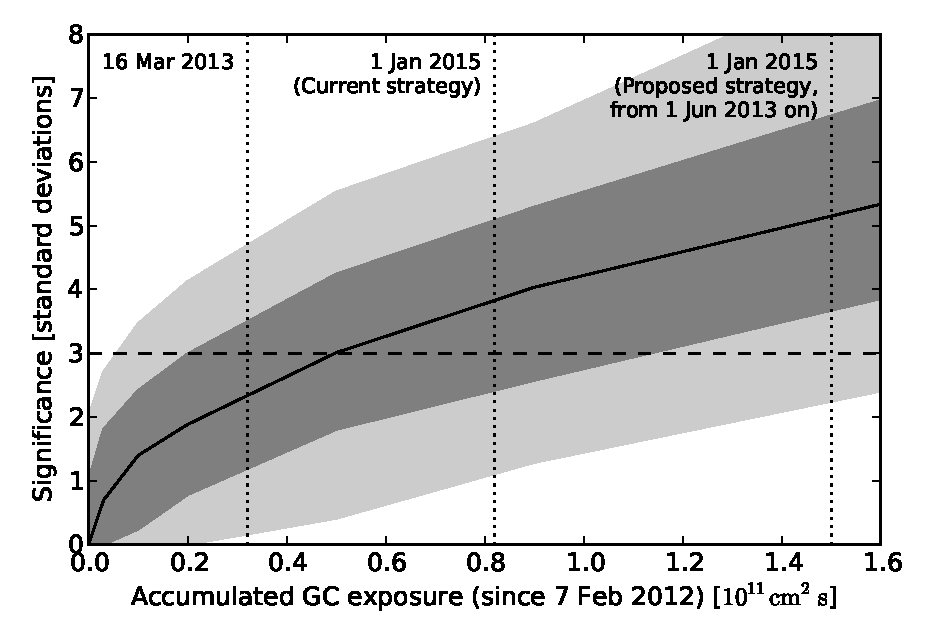
\includegraphics[width=0.8\linewidth]{plots/projection.eps}
    \vspace{-0.5cm}
  \end{center}
  \caption{Evaluation of mixed observation strategy. \emph{Top panel:}
    Effective energy resolution in different sky regions. \emph{Central
      panel:} change in exposure relative to standard survey
    mode. \emph{Bottom panel:} Figure of merit for gamma-ray line searches in
    different sky regions.}
  \label{fig:option}
\end{figure}


\begin{figure}[h]
  \begin{center}
    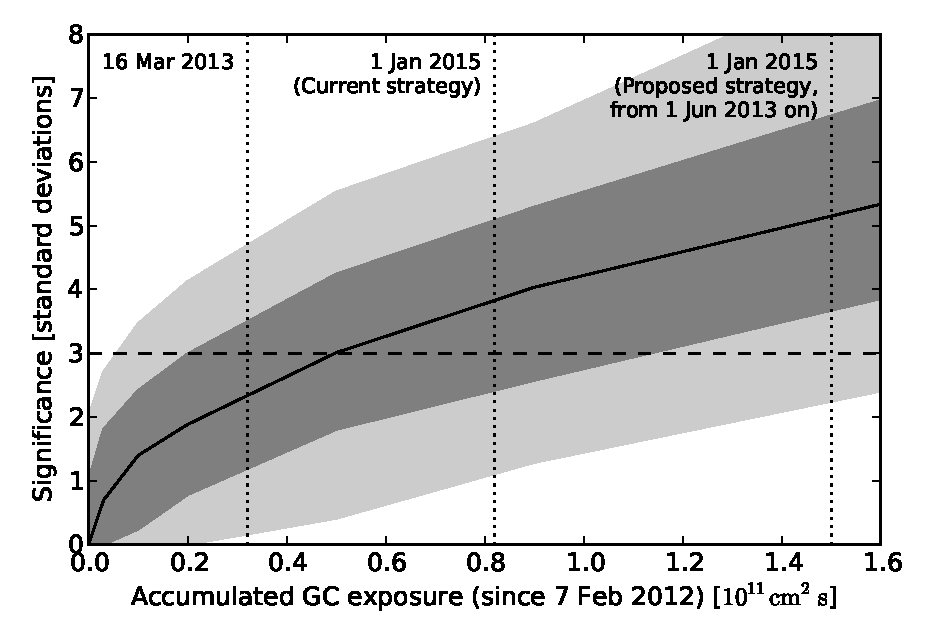
\includegraphics[width=0.8\linewidth]{plots/projection.eps}
    \vspace{-0.5cm}
  \end{center}
  \caption{Expected growth in signal significance as new data are accumulated,
    starting from 7 February 2012. The shaded bands show $68\%$ and $95\%$
    C.L., and are derived from a Monte Carlo simulation. For the predictions,
    we adopt the signal and background fluxes as they were measured prior to 7
    February 2012. The second and third vertical dotted lines indicate
    respectively the accumulated exposure until end of 2014 when the
    observation strategy remains unchanged, and when the mixed observation
    strategy is adopted starting from June 2013 (see Fig. 2)}
  \label{fig:projection}
\end{figure}




\section{Discussion and Conclusion}
\label{sec:Conclusion}

In this paper, we search the publicly available LAT data for any trends or
correlations that might indicate an instrumental origin for the spectral
feature at $\sim$130 GeV towards the GC \citep{Bringmann:2012, Weniger:2012, linepaper}. 
After addressing the following concerns, we find no evidence that the 130 GeV
feature is spurious. 
\medskip

\emph{The Galactic center is bright and has a hard spectrum.} On degree
scales, the GC surface brightness is less than a factor of 2 brighter than the
inner Galactic plane.  The inner plane provides an order of magnitude more
photons, and shows no sign of a 130 GeV bump.  Even larger samples (all limb
photons, all non-limb non-GC photons) also show no significant signal.  The GC has a hard
spectrum, and at TeV energies the
GC is brighter than the surrounding plane, but even if \emph{all} events above
300 GeV (assuming a hard spectrum $dN/dE\sim E^{-2}$) were incorrectly remapped
to 130 GeV, there would not be enough photons to explain the GC signal.

\emph{Observations of the GC have a restricted range of instrumental incidence
  angles.}  It is true that the survey strategy, orbital precession, and solar
panel alignment cause a non-trivial mapping of GC events onto $(\theta, \phi)$
as a function of time of year.  Specifically, they occur near the $x-z$ plane
($\phi=0$ or 180) when the Sun is near the GC or anti-center.  However, the GC
line events are drawn from the full range of $\theta$, $\phi$, and $t$.  The
limb line events are broadly distributed in $\theta$, $\phi$, and $\ell$, with
times corresponding to pointed observations at large zenith angle.  There is no
evidence that the distribution of line events deviates from expectations.

\emph{There are excess line events in the limb data for some incidence angles.}
For a small subset of the limb data with large rocking angle (when the limb may
be seen at small incidence angles) and a particular incidence angle range
around $30\degree$ to $45\degree$, we find a marginally significant 130 GeV feature
(above $3\sigma$).  
%This feature is not observed in limb events at other incidence angles.  
The majority of events with incidence angle $30\degree$ to
$45\degree$ are \emph{not} from the Earth limb, and we find no 130 GeV
feature in this much larger sample of events at these incidence angles.  If the
limb line events are an artifact, they must conspire to only appear when the
LAT is positioned at high rocking angle. 

\emph{The bump in the limb data might result from an energy mapping error.}
We propose a simple model for an error in the mapping from true photon energy
to reported energy.  This model reproduces the shape of the limb line feature
at 130 GeV and the dip at slightly higher energy, and has a local significance
of 4.7$\sigma$.  A modest amount of additional limb data would tell us if the
limb feature is a statistical fluke.  If the limb feature persists, it raises
serious concerns about the \texttt{Pass 7} processing of $E > 100$ GeV events.
\medskip

Additional limb data are available from the commissioning
period.  The Launch \& Early Operations (LEO) data were
taken during the first 60 days of the mission. Combined with
a dedicated Earth-limb observation in September 2008, this
provides $\sim$250 hours total livetime on the Earth
limb~\cite{FermiLimb}.

With \texttt{Pass 6} \texttt{diffuse} class events,
\cite{FermiLimb} has analyzed the spatial morphology and the
energy spectrum of the Earth limb sample,
which contains 218 photons above 100 GeV and 16 photons
above 500 GeV. The energy spectrum 
is a power-law with spectral index $2.79\pm
0.06$ for 3-500 GeV photons (Fig.~2 of \cite{FermiLimb}),
which is consistent with the primary cosmic-ray spectral
index $2.75\pm 0.03$.\footnote{The Earth limb photon above 10
  GeV from CR interactions in the upper atmospheric
  layers do not suffer large energy loses and the cosmic-ray
  primaries at this energy are unaffected by the Earth's
  magnetic fields. The Earth limb photons should have a
  spectral index close to that of the primary cosmic
  rays~\cite{FermiLimb}. } 

The spectrum of the Earth limb photons provided by
\citep{FermiLimb} does not show any significant feature at
130 GeV. If improved processing of the limb photons does not
replicate the line or the "energy mapping error" we found for a
subsample of the limb photons during the normal survey mode,
it can be dismissed as a statistical fluke.  If it
reappears, a deeper investigation into its cause will be necessary.

Even then, it is a challenge to understand how such an
instrumental feature could be mapped so precisely onto a
localized region within $5-10\degree$ of the GC.  The GC is
not near the path of the orbital pole, nor its axis of
precession.  The orbital phase, precession, Earth's orbit,
and time of year are all well mixed by the few $\times10^4$
orbits and 25 precession cycles over 1500 days.  We have
shown that the events in question are drawn from every part
of event and spacecraft parameter space available in the
public files. 

In summary, we find no significant instrumental systematics that could
plausibly explain the excess Galactic center emission observed at 130 GeV. 

\vskip 0.15in {\bf \noindent Note added:} During the final stages of this
work we became aware of another group discussing instrumental indications in
the Earth limb data~\cite{TempelSoon}.

\vskip 0.15in {\bf \noindent Acknowledgments:} We thank Neal
Weiner, Dan Hooper, and Jesse Thaler for helpful discussions. We acknowledge the use of
public data from the \Fermi\ data archive at
\texttt{http://fermi.gsfc.nasa.gov/ssc/}.  M.S. and
D.P.F. are partially supported by the NASA Fermi Guest
Investigator Program. Support for the work of M.S. was
provided by NASA through Einstein Postdoctoral Fellowship
grant number PF2-130102 awarded by the Chandra X-ray Center,
which is operated by the Smithsonian Astrophysical
Observatory for NASA under contract
NAS8-03060. C.W. acknowledges partial support from the
European 1231 Union FP7 ITN INVISIBLES (Marie Curie Actions,
PITN-GA-2011-289442).  This research made use of the NASA
Astrophysics Data System (ADS) and the IDL Astronomy User's
Library at Goddard (Available at
\texttt{http://idlastro.gsfc.nasa.gov}).

\clearpage
\bibliography{whitepaper}

\end{document}
